\chapter{Implementation}
The fifth chapter, \textit{Implementation}, describes the actual implementation of the training of the machine learning model used for classifying the transportation of the user and of the application to determine the parking position of the user's car. 
In the first section, \textit{Architecture}, the architecture of the developed system is presented and explained.
The second section, \textit{Technologies}, outlines the technologies used in the implementation of the system.
In the third section, \textit{Details of Implementation}, several noteworthy code excerpts of the application, the implementation of the machine learning workflow and the server component are presented.

\section{Architecture}

\begin{figure}[h]
    \centering
    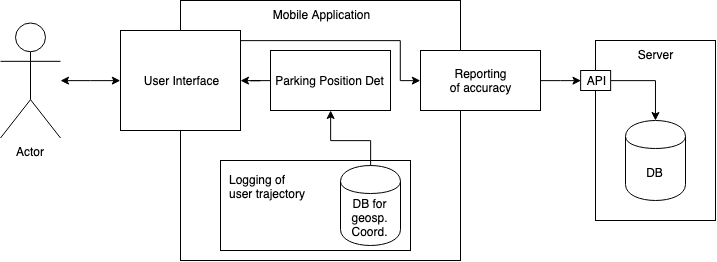
\includegraphics[width=0.9\textwidth]{images/architecture.png}
    \caption{Architecture of Developed System}
    \label{fig:architecture}
\end{figure}


The system is centered around the developed mobile application. Figure \ref{fig:architecture} visualises the architecture. The arrows represent the data flow.  The mobile application consists of four components: the user interface, the logging of  the user's trajectory, the determination of the parking position of the user's car and the reporting of the accuracy. The user interface presents all necessary data to the user and the user can perform actions through it. The component that logs the user's trajectory saves the coordinates together with the current timestamp of the coordinates and other meta information in a database on the phone. The component that determines the parking position of the user's car reads the logged trajectory of the user and performs the determination algorithm completely on device. The user can proactively report the accuracy of the determined parking position using the corresponding component. This component sends the accuracy and other meta data, but no sensitive data such as any actual location, to the server component. The data is securely transmitted via the HTTPS protocol. The server component consists of an API which accepts the data sent by the mobile application and stores it in a database.

\section{Technologies}

\paragraph{Swift} Swift\footnote{Swift: \url{https://swift.org/about/}, (online: last accessed October 19, 2019)} is a general-purpose language developed by Apple Inc and being open-source since 2015. It is mainly developed to be used on Apple's platforms iOS, macOS, iPadOS, watchOS and tvOS, but can be used on other platforms as well. Its design focuses on safety, performance and expressiveness. It implements these by the avoidance of null values, direct compilation for each platform and a strict syntax. \cite{apple:swift}

\paragraph{Alamofire} Alamofire\footnote{Alamofire: \url{https://github.com/Alamofire/Alamofire}, (online: last accessed October 19, 2019)} is an HTTP networking library. It is written in Swift. In this Bachelor thesis it is used to report the accuracy of the determined parking position to the server component. \cite{alamofire}

\paragraph{Realm Database} Realm Database\footnote{Realm Database: \url{https://realm.io/products/realm-database/}, (online: last accessed October 19, 2019)} is an open source database management system with a focus on mobile platforms. Its core is written in C++ which enables a high performance. It can perform more than twice as many queries per second than the native solution of iOS called Core Data\footnote{Core Data: \url{https://developer.apple.com/documentation/coredata}, (online: last accessed October 19, 2019)}.  Realm Database is used in the application to store the trajectory of the user on device. \cite{realm}

\paragraph{MapKit} MapKit\footnote{MapKit: \url{https://developer.apple.com/documentation/mapkit}, (online: last accessed October 19, 2019)} is a framework to embed maps in an iPhone application. It is developed by Apple. In this Bachelor thesis, the framework is used to present the user's location and the determined parking position on a map. \cite{apple:MapKit}

\paragraph{Jupyter Notebook} Jupyter Notebook\footnote{Jupyter Notebook: \url{https://jupyter.org/}, (online: last accessed October 19, 2019)} is an open-source web application that provides an environment to write code in a live context for a variety of languages and to present the code and its computational results. Jupyter Notebook is used in this Bachelor thesis to implement the machine learning training \cite{jupyter}

\paragraph{Node.js} Node.js\footnote{Node.js: \url{https://nodejs.org/en/about/}, (online: last accessed October 19, 2019)} is an asynchronous event-driven JavaScript runtime. It is used to build network applications. In this Bachelor thesis it is used to build the server component of the accuracy reporting. \cite{node}

\paragraph{Scikit-learn} Scikit-learn\footnote{Scikit-learn: \url{https://scikit-learn.org/stable/}, (online: last accessed October 19, 2019)} is a Python library which implements a variety of machine learning algorithms. This Bachelor thesis uses Scikit-learns implementation of XGBoost and Multylayer Perceptron Neural Networks to classify the transportation modes of a user's spatial trajectory. \cite{scikit-learn}

\section{Details of Implementation}

The application is implemented for iPhones running the operating system iOS 13, the machine learning model training is implemented using Jupyter Notebooks and the server component is implemented using Node.js. All source code can be found in their repositories\footnote{Repository of implemented machine learning notebooks: \url{https://github.com/greenBene/ba-ml-model}, (online: last accessed October 19, 2019)} \footnote{Repository of implemented application: \url{https://github.com/greenBene/ba-parking-position-determination/}, (online: last accessed October 19, 2019)} \footnote{Repository of implemented server: \url{https://github.com/greenBene/ba-server}, (online: last accessed October 19, 2019)}.

Figure \ref{fig:ui} shows the three main views of the application. The left view presents the view the user sees when they start the application. It shows the current position of the user on a map and a button to initiate the determination of the parking position. The middle view pictures the status of the application if a parking position is determined. It shows the location of the car and the location of the user on a map. Also, it presents more detailed information about the location of the car, such as the address where it is parked and the relative distance and altitude between the user's location and the determined parking position. If data regarding the floor of the car is available, it is shown as well. The user can trigger three actions via buttons on this screen. First, they can start a navigation towards the position of the user's car in the standard navigation software Apple Maps. Second, they can go back to the previous screen, ''Map View - Loading'', via the reverse button. Third, they can report the accuracy of the application. The right view shows the interface of the application after the user initiates the reporting of the accuracy. An explaining text and the shared information are shown in the view. The user can report the presented data using the button at the bottom. 

\begin{figure}[h!]
\begin{minipage}{.33\textwidth}
  \centering
  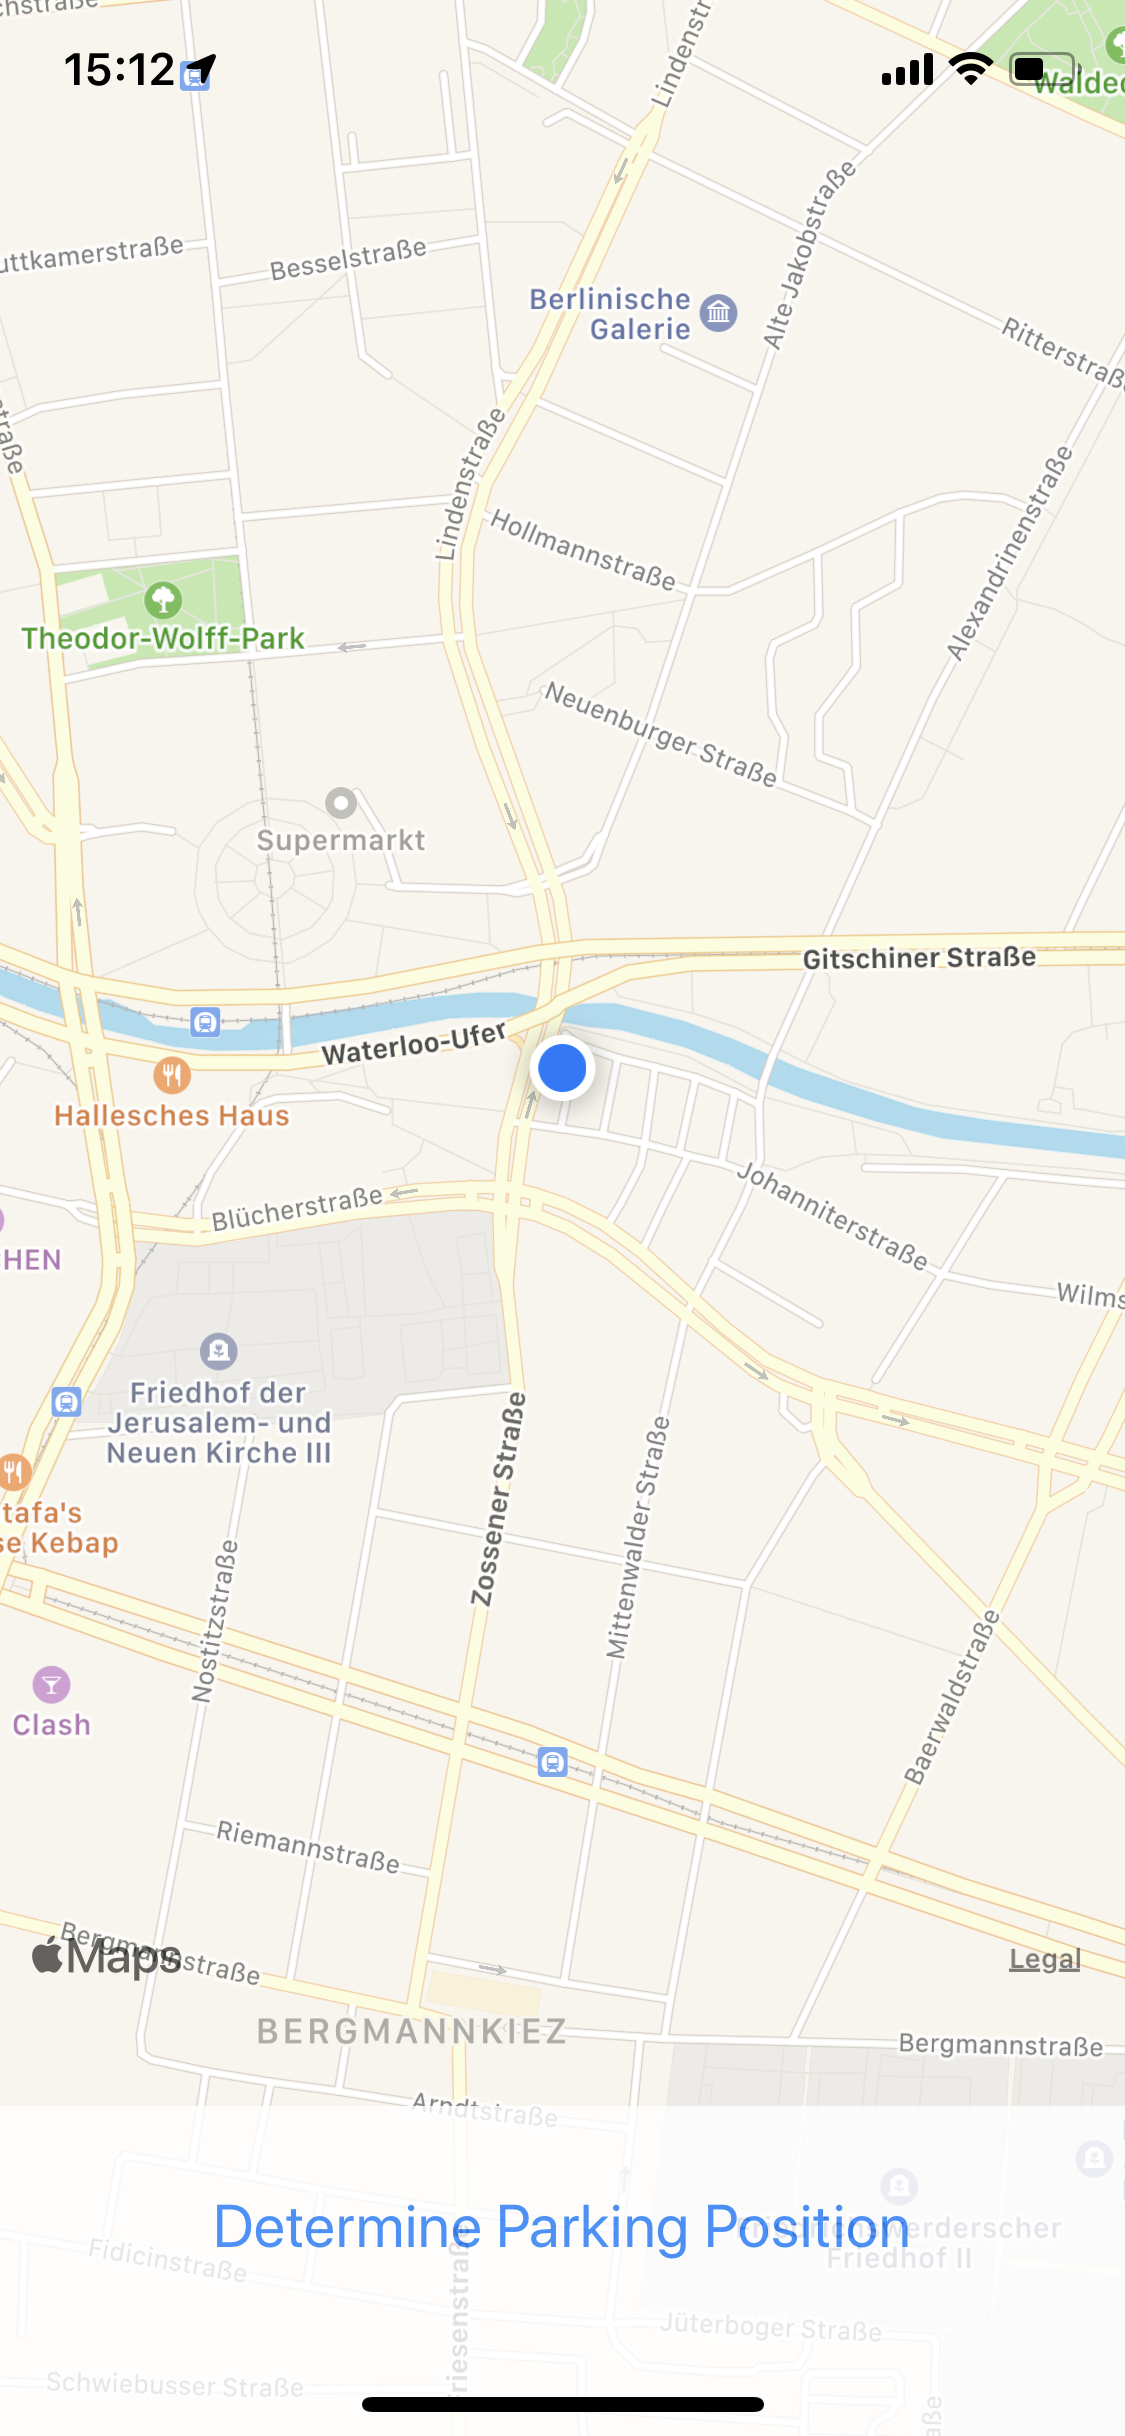
\includegraphics[width=.9\linewidth]{images/App/start.png}
\end{minipage}%
\begin{minipage}{.33\textwidth}
  \centering
  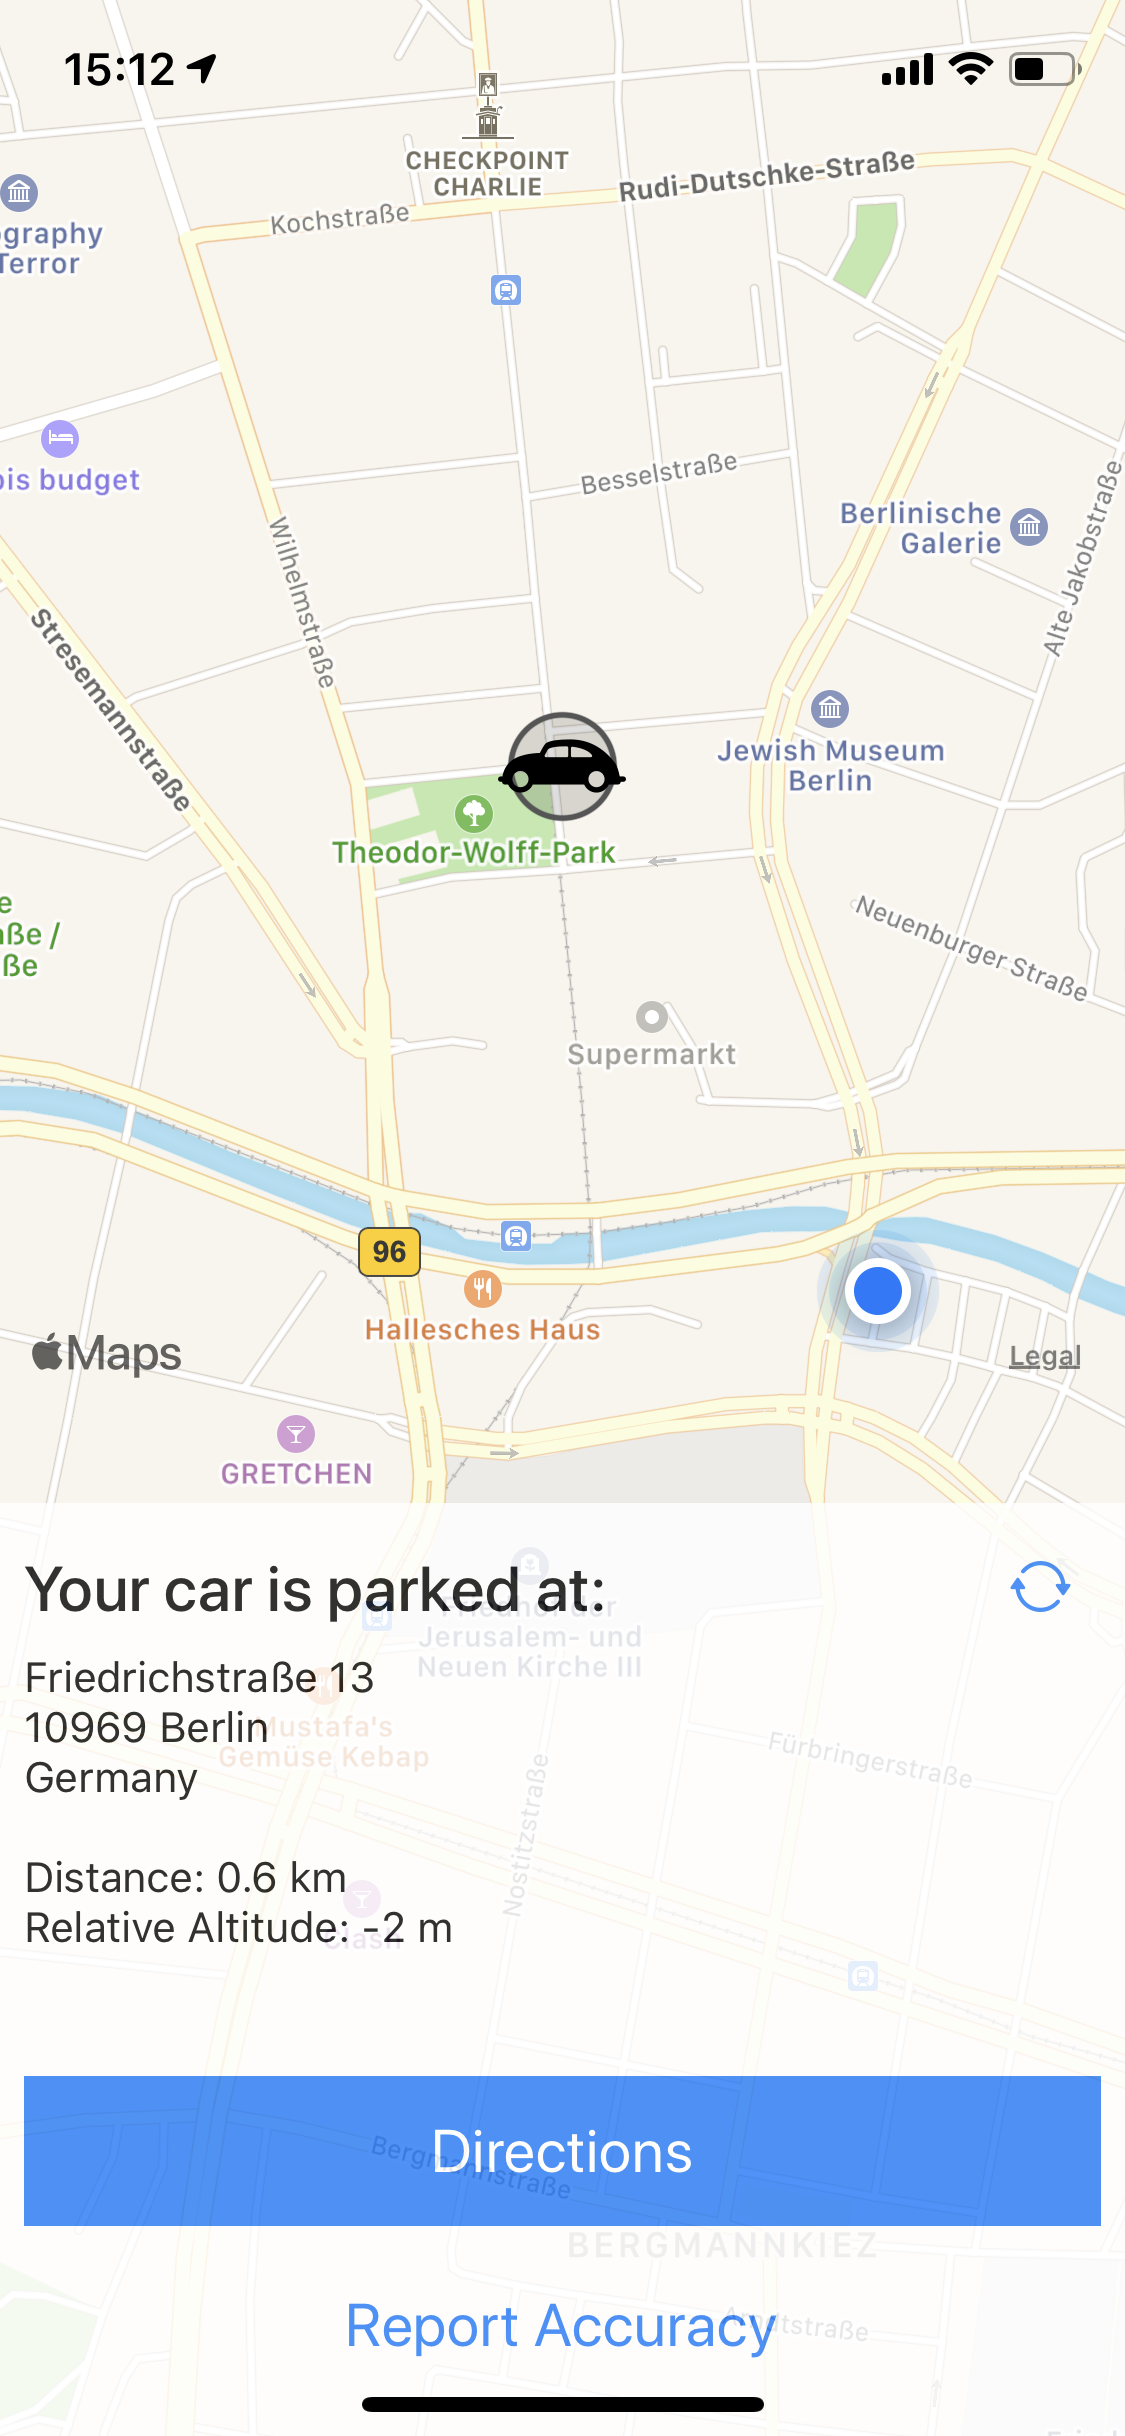
\includegraphics[width=.9\linewidth]{images/App/detail.png}
\end{minipage}
\begin{minipage}{.33\textwidth}
  \centering
  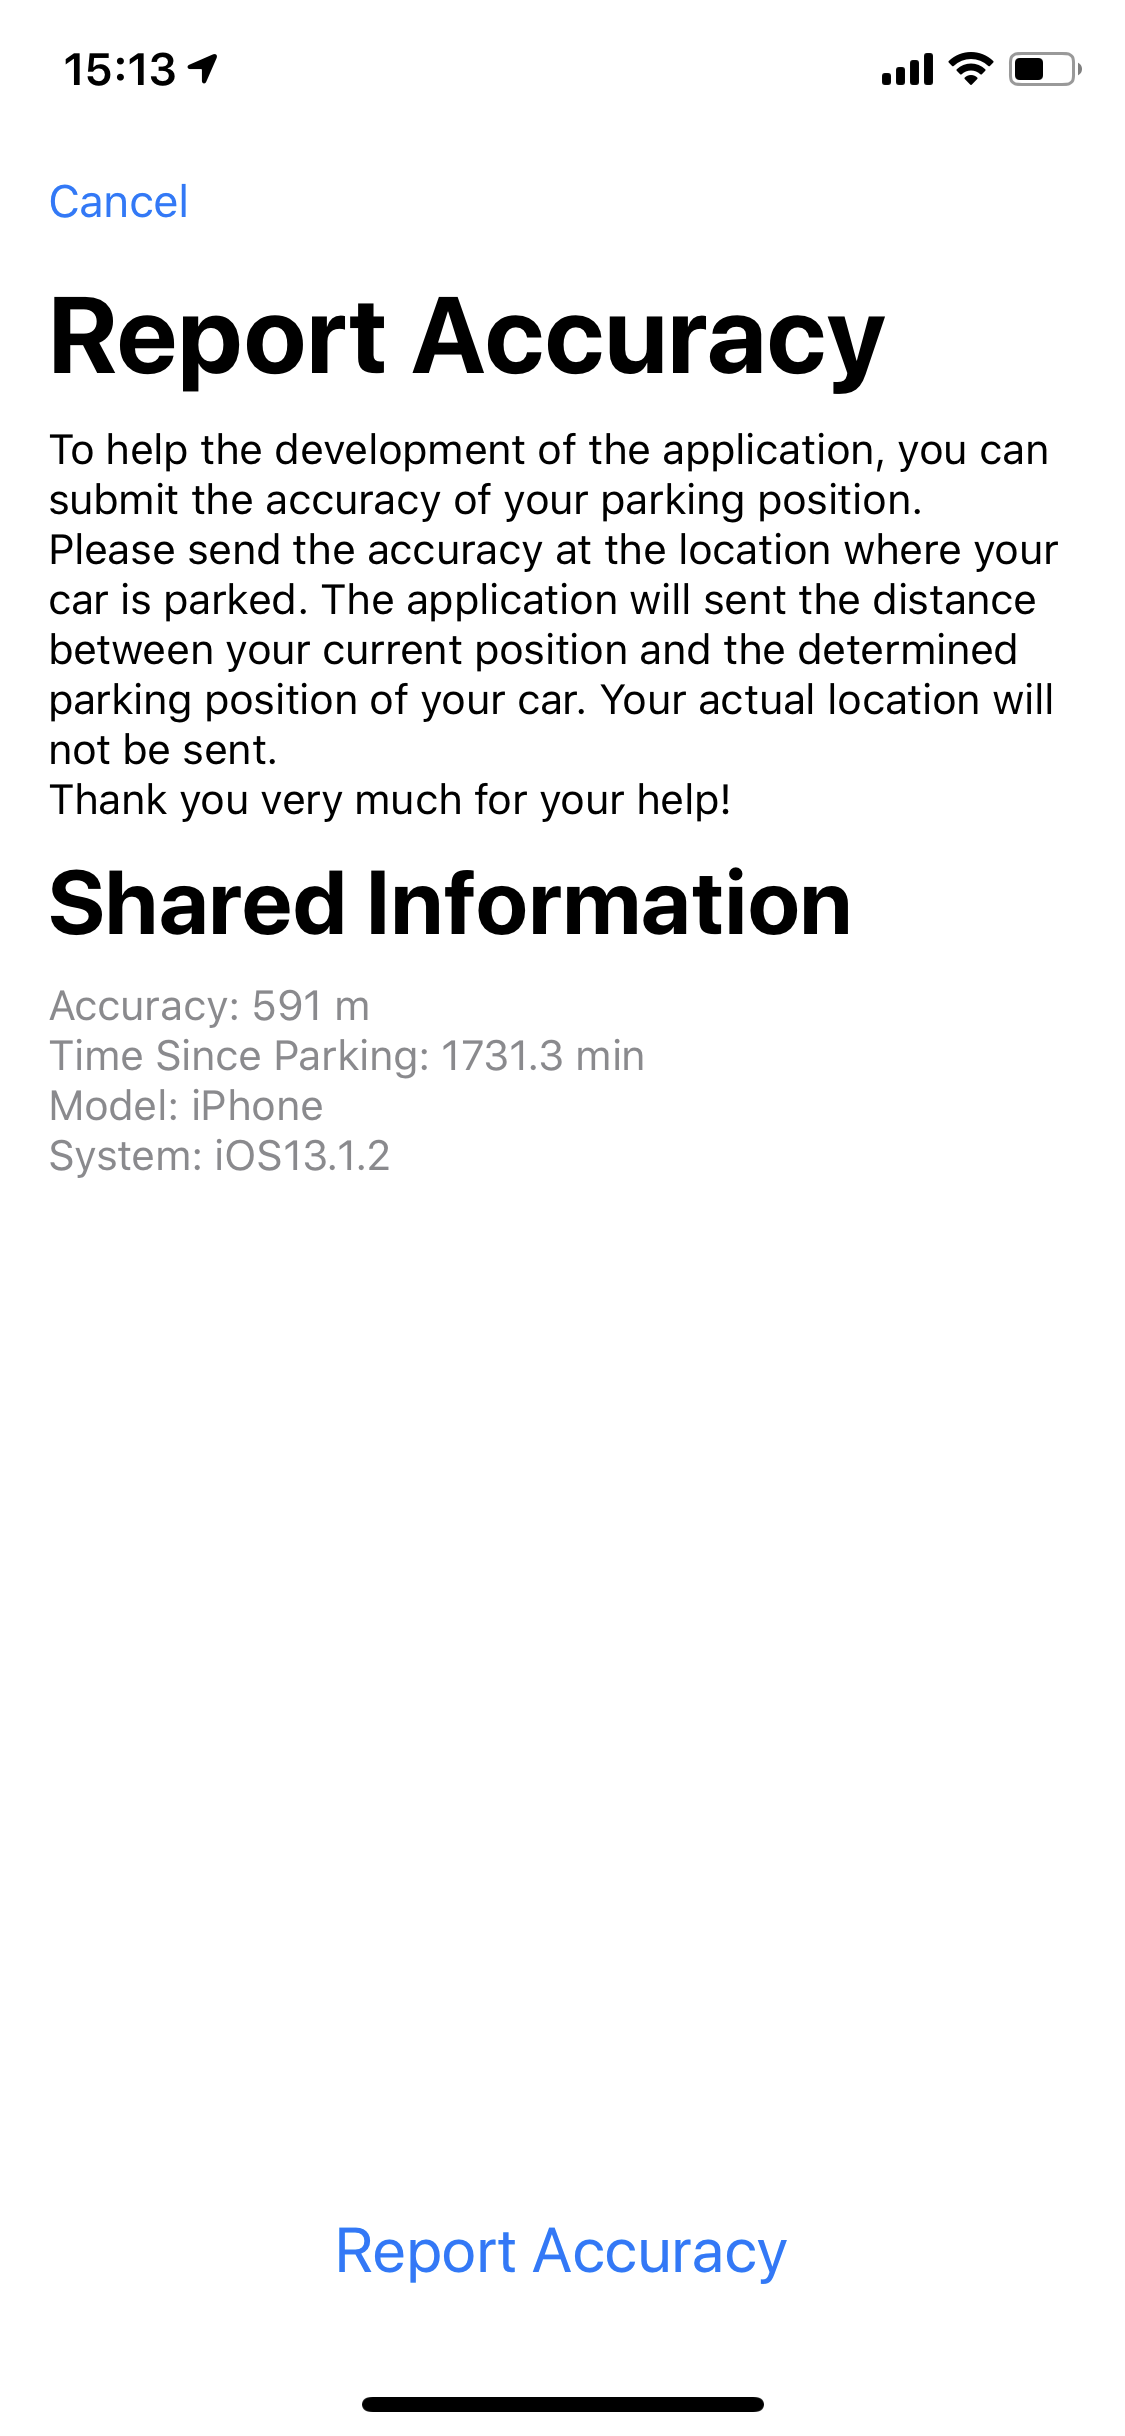
\includegraphics[width=.9\linewidth]{images/App/feedback.png}
\end{minipage}
\caption{The Three Main Views of the Implemented Application. MapView - Loading (left), MapView - Parking Position Determined (middle), and Report Accuracy (right).}
\label{fig:ui}
\end{figure}
\newpage

\paragraph{Training of XGBoost Classifier} Source Code \ref{code:xgb_train} shows the implementation of the training of the XGBoost classifier. First, a XGBoost classifier object is created and possible parameters are defined in a dictionary. These parameters are chosen because they show the best results using three-fold cross-validation. The model is then trained for all possible combinations of the parameter space and the best model is chosen. 

\begin{lstlisting}[style=py, caption={Train XGBoost Classifier}, label={code:xgb_train}]
xgb = XGBClassifier()

parameter_space = {
    'objective': ['binary:logistic'],
    'learning_rate': [0.2],
    'max_depth': [10],
    'min_child_weight': [8],
    'subsample': [0.4],
    'n_estimators': [30]
}

from sklearn.model_selection import GridSearchCV

clf = GridSearchCV(xgb, parameter_space, n_jobs=-1, cv=3, verbose=10)
clf.fit(X_train, y_train)

print('Best parameters found:\n', clf.best_params_)
\end{lstlisting}{}


\paragraph{Determine Parking Position Algorithm Implementation} Source Code \ref{code:detParkPosImpl} shows the implementation of the algorithm to determine the parking position of the user's car. The whole trajectory of the user is loaded and the noise of the sensors is removed. The cleaned trajectory is cut into trips based on the stay points of the user. These trips are then labeled with their transportation modes and based on this, parking position candidates are computed. The most recent candidate is returned as the parking position.

\begin{lstlisting}[style=swift, caption={Implementation of Algorithm to Determine Parking Position of the User's Car}, label={code:detParkPosImpl}]
func determineParkingPosition() throws -> (CLLocation, [StayPoint]){
        // Load trajectory
        var trajectory = loadTrajectory()
        
        // Remove noise
        trajectory = removeNoise(coords: trajectory)
        
        let stayPoints = getStayPoints(locations: trajectory, distThresh: DISTANCE_THRESHOLD, timeThresh: TIME_THRESHOLD)
        
        // Cut it into trips based on stay points
        let trips = cutIntoTrips(stayPoints: stayPoints, trajectory: trajectory)
        
        let classifier = trans_mode()
        
        for trip in trips.reversed() {
            let features = try featureExtraction(locations: trip)
            
            let output = try classifier.predictions(inputs: features)
            
            do {
                guard let loc = try determineParkingPosCandidate(trajectory: trip, labels: output) else {
                    continue
                }
                return (loc, stayPoints)
                
            } catch {
            
            }
        }
        throw ClassificationError.noParkingLocationDetermined
    }
\end{lstlisting}

\paragraph{Determine Stay Points - Implementation}
Source Code \ref{code:detStayPointsImpl} shows the implementation of the stay point detection. This algorithm is adapted in most parts from \cite{li2008mining} but it is adapted in two places. First, as mentioned in the fourth chapter, \textit{Design}, the original algorithm has a potential infinity loop. This is fixed by moving the line i = j from the original line 25 to line 36. Also, when the algorithm finishes, the last potential start of a stay point is added to the list of stay points. This is implemented so that the most recent trip can be used for determining the parking position of a car. 

\begin{lstlisting}[style=swift, caption={Determine Stay Points - Implementation}, label={code:detStayPointsImpl}]
private func getStayPoints(locations: [CLLocation], distThresh: Double, timeThresh:Double) -> [StayPoint] {
        var i = 0; let pointNum = locations.count;
        var stayPoints: [StayPoint] = Array()
        
        while i < pointNum {
            var j = i + 1
            while j < pointNum {
                let p_i = locations[i]
                let p_j = locations[j]
                let dist = p_i.distance(from: p_j)
                
                if dist > distThresh {
                    let timeDelta = p_j.timestamp.timeIntervalSince(p_i.timestamp)
                    if timeDelta > timeThresh {
                        let meanLoc = computeMeanCoordinate(coords: Array(locations[i...j]))
                        
                        stayPoints.append(
                            StayPoint(lat: meanLoc.latitude, lon: meanLoc.longitude,
                                                    arrivalTime: p_i.timestamp, leaveTime: p_j.timestamp,
                                                    distThresh: distThresh, timeThresh: timeThresh)
                        )
                    }
                    break
                }
                j = j+1
            }
            
            if(j >= pointNum){
                stayPoints.append(
                    StayPoint(lat: locations[ i ].coordinate.latitude, lon: locations[ i ].coordinate.longitude,
                                            arrivalTime: locations[ i ].timestamp, leaveTime: locations[ i ].timestamp,
                                            distThresh: 0, timeThresh: 0)
                )
            }
            
            i = j // Algorithm in source lacks this line. Otherwise potential infinity loop.
        }
        
        let firstLocation = locations[0]
        stayPoints = [StayPoint(lat:firstLocation.coordinate.latitude , lon: firstLocation.coordinate.longitude,
                                arrivalTime: firstLocation.timestamp, leaveTime: firstLocation.timestamp, distThresh: 0, timeThresh: 0)] +
                     stayPoints
        
        return stayPoints
    }
\end{lstlisting}{}

\paragraph{Server: Handling of Reported Accuracy} Source Code \ref{code:server} shows the function of the server that handles incoming reports of accuracy. First, it parses the incoming message and retrieves the transmitted values. Second, it ensures that the necessary values are set. Third, if the data is valid, it inserts the values into a table of a MySQL database. After the successful insertion or after any error, the server sends an appropriate HTTP code to the client.


\begin{lstlisting}[style=JavaScript, caption={Server: Handling of Reported Accuracy}, label={code:server}]
app.post("/post", function(req, res){
  var body = req.body;

  var model = body.model;
  var os = body.os;
  var timeSinceParking = body.timeSinceParking;
  var accuracy = body.accuracy;
  var test = body.test;

  console.log("Received message");

  if(model === undefined || os === undefined
    || timeSinceParking === undefined
    || accuracy === undefined){

    res.sendStatus(400);
    return;
  }

  var sql = "INSERT INTO accuracy VALUES (0, current_timestamp(), '" + model +  "', '" + os + "', " + timeSinceParking +  ", " + accuracy +  ");"

  con.query(sql, function (err, res) {
    if (err){
      console.log(err);
      res.sendStatus(500);
    }

    });

  res.sendStatus(200)
});
\end{lstlisting}{}